\begin{figure}
    \centering
    \begin{subfigure}[b]{0.485\linewidth}
        \centering
        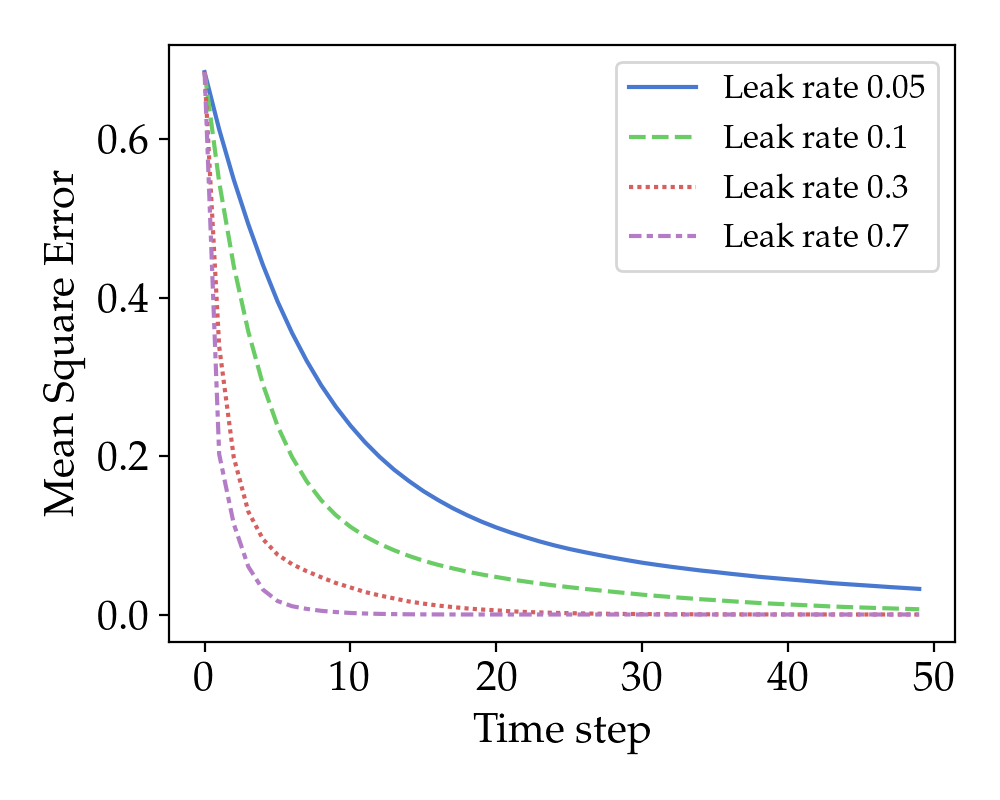
\includegraphics[width=\linewidth,height=\linewidth,keepaspectratio]{img/esn_starting_conditions.png}
        \caption{First method: divergence between reservoirs}
        \label{fig:memory_esn_start}
    \end{subfigure}
    \vskip\baselineskip
    \begin{subfigure}[b]{0.485\linewidth}
        \centering
        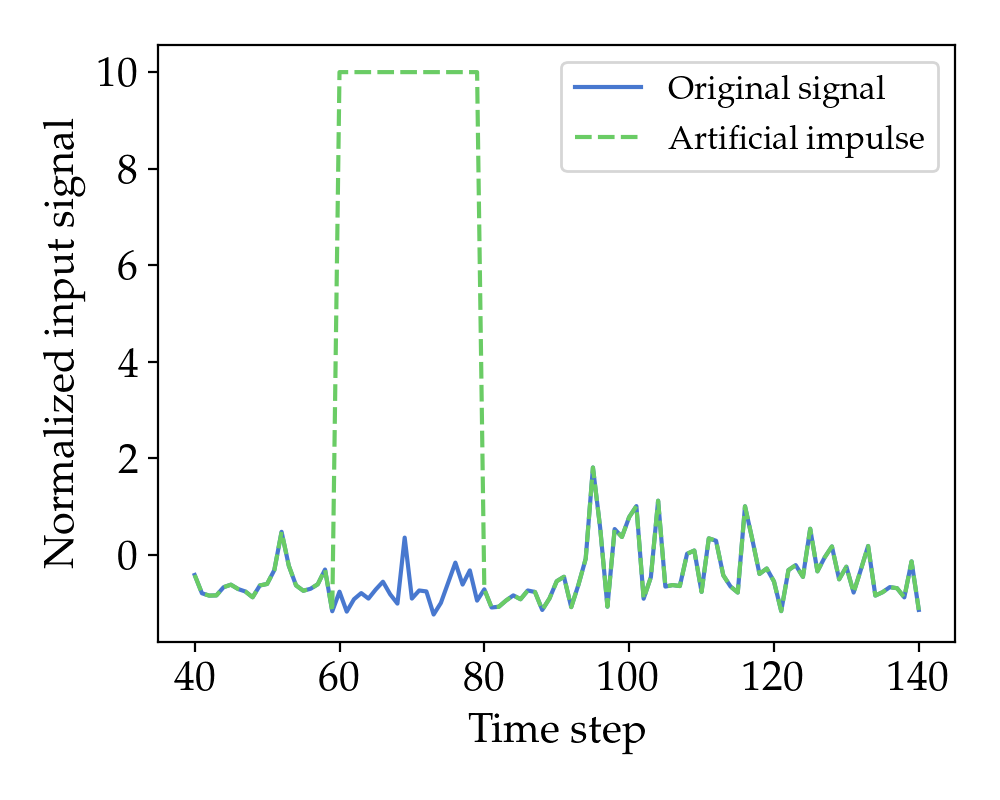
\includegraphics[width=\linewidth,height=\linewidth,keepaspectratio]{img/input_impulse.png}
        \caption{Second method: applying an artificial impulse}
        \label{fig:memory_input_impulse}
    \end{subfigure}
    \hfill
    \begin{subfigure}[b]{0.485\linewidth}
        \centering
        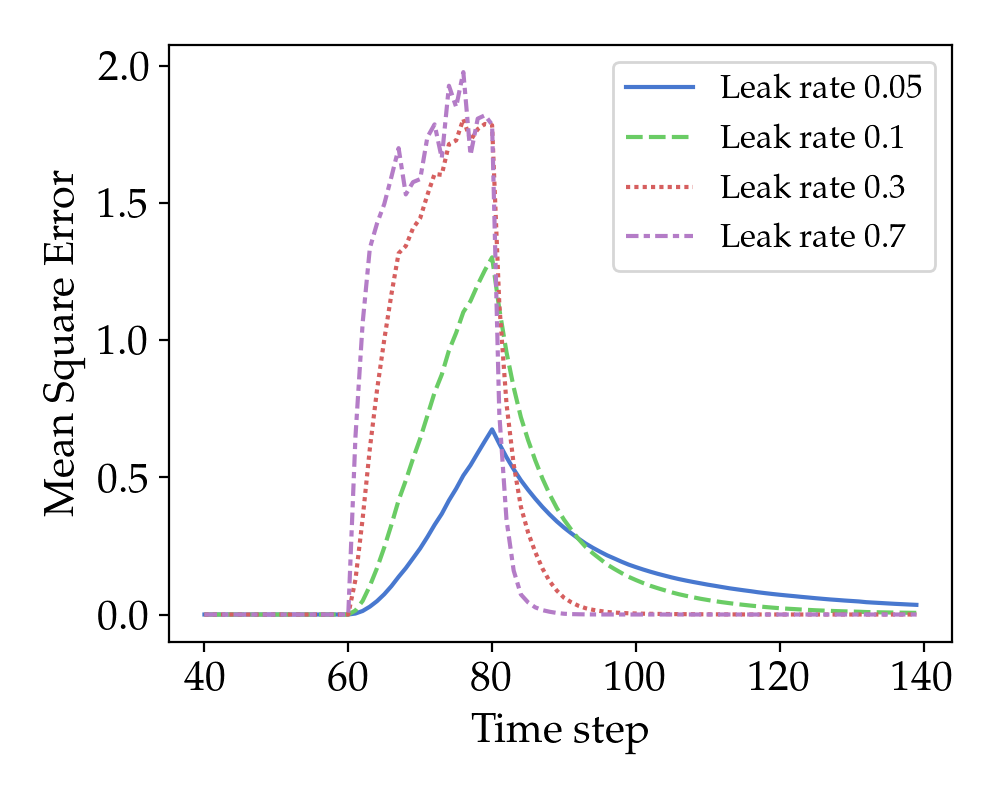
\includegraphics[width=\linewidth,height=\linewidth,keepaspectratio]{img/esn_impulse.png}
        \caption{Second method: divergence between reservoirs}
        \label{fig:memory_esn_impulse}
    \end{subfigure}
    \caption[Two methods for testing the fading memory property of a reservoir, demonstrated using a \acrshort{esn}.]{
            These figures show experimental data from testing the fading memory property of an \acrshort{esn} as described in Subsection \ref{sec:fading_memory}. 
            Both experiments use a reservoir of 100 nodes with randomly initialized weights. 
            For stability, we normalized the weights to have a spectral radius below 1.25 \citep{caluwaerts_design_2014}.
            As input data, we used the California Housing regression dataset \citep{kelley_pace_sparse_1997} which can be found in the sklearn Python package.
            (\subref{fig:memory_esn_start}) The divergence in reservoir state between two runs of the same reservoir with identical inputs and different starting state vectors. 
            The starting states are sampled from a uniform distribution between -1 and 1.
            The disparity between the reservoirs is measured by the MSE between their respective state vectors (Equation \ref{eq:MSE}).
            (\subref{fig:memory_input_impulse}) An artificial impulse with an amplitude of ten times the standard deviation of the original signal is applied between time steps 60 and 80.
            (\subref{fig:memory_esn_impulse}) The divergence in reservoir state between two runs of the same reservoir using identical starting conditions. One run receives an artificial impulse between time step 60 and 80 on all input dimensions, as depicted by Subfigure \subref{fig:memory_input_impulse}.
    }
    \label{fig:fading_memory_experiments}
\end{figure}

